\documentclass[12pt,a4paper,article,english,firamath]{nsi}
\pagestyle{empty}
\setfontfamily{\brettley}{Cursive standard}[Scale=1.5]
\begin{document}
\titre{Find your figure}
\classe{Euro 1\ere}
\maketitle
\subsection*{Description 2}
{\brettley
Draw two perpendicular lines. Draw a circle whose diameter is the line segment of endpoints their point of intersection and another point on one of the two lines. Draw another circle with a diameter twice as long, on the second line. Draw a line parallel to the first one and passing through the intersection of this circle and the second line. Draw a line passing through the intersections of these two circles.}\\[1em]


\begin{tikzpicture}
    \draw[lightgray](0,0)--(\linewidth,0);
\end{tikzpicture}


\subsection*{Figure 2}
\begin{center}
    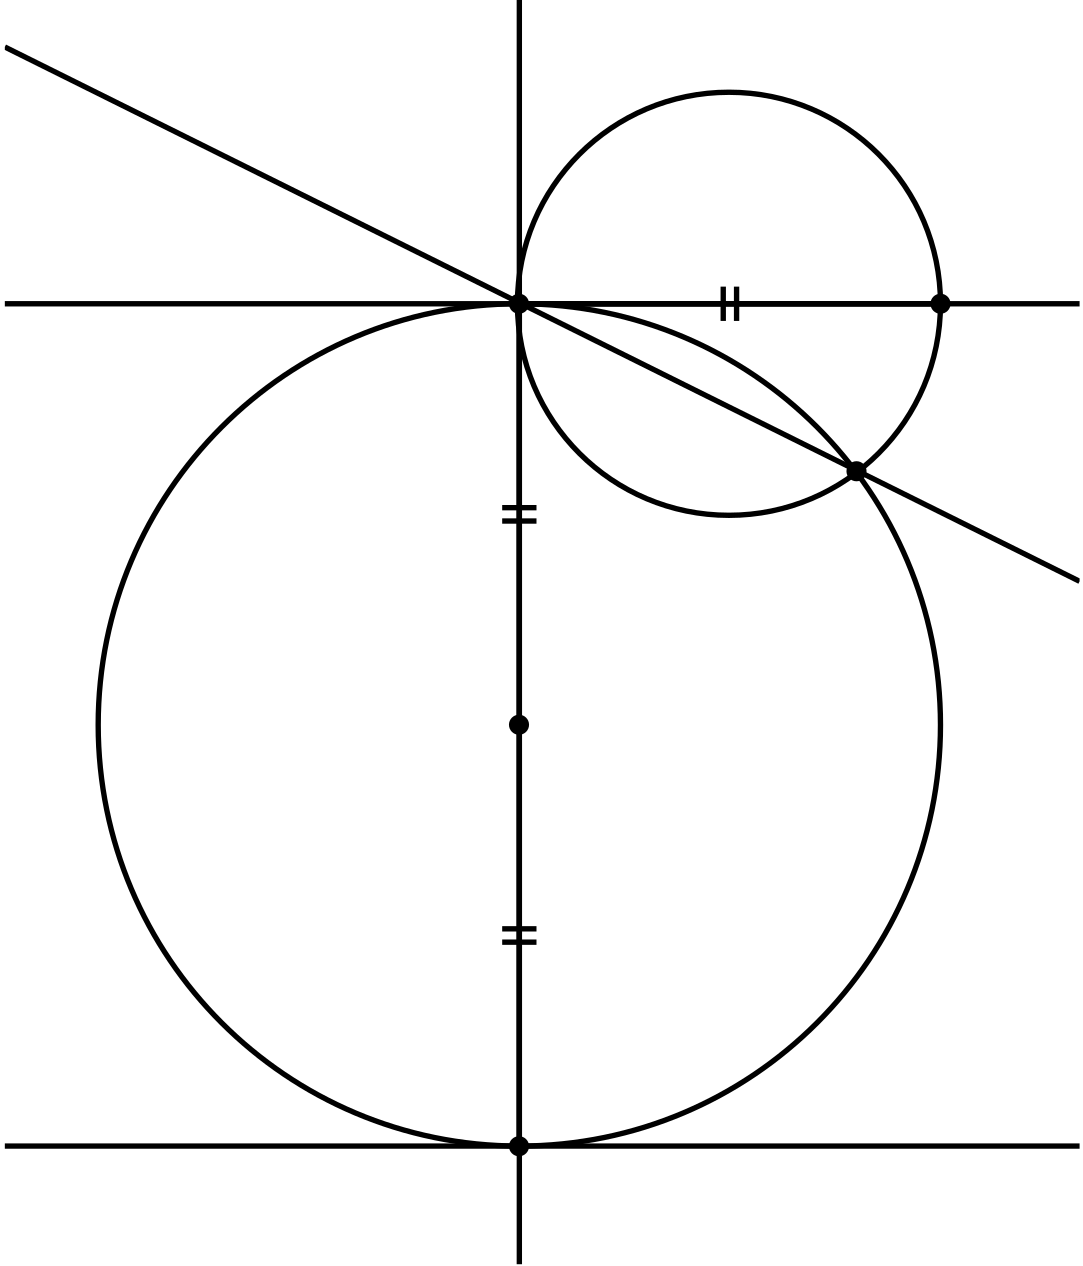
\includegraphics[height=12cm]{img/fig02.png}
\end{center}
\end{document}